\documentclass[final,t]{beamer}
\mode<presentation>{ \usetheme{Major} }
  \usepackage{times}
  \usepackage{amsmath,amsthm, amssymb, latexsym}
  \boldmath
  \usepackage[english]{babel}


\usepackage{tikz}
\usetikzlibrary{positioning,shadows,arrows,shapes,calc,backgrounds}

\definecolor{forestgreen}{RGB}{34,139,34}
  
  	\usepackage{relsize}
  	\usepackage{multirow}
	%\usepackage{qtree}
	\usepackage{stmaryrd}
	\usepackage{booktabs}
%  \usepackage[font=small,format=plain,labelfont=bf,up,textfont=it,up]{caption}
  	\usepackage[font=scriptsize,labelfont=scriptsize,bf]{caption}
  	\usepackage[latin1]{inputenc}
  	\usepackage[orientation=landscape,size=a1,scale=1.4,debug]{beamerposter}
  	\usepackage{color,listings}
  	\usepackage{calc,xcolor}
        
\definecolor{lightblue}{rgb}{.85,.85,1} % 217 217 255
\definecolor{lightorange}{rgb}{1,.8,.6} % 255 204 153
\definecolor{lightgreen}{rgb}{.77,.91,.5} % 196 232 128
\definecolor{lightyellow}{rgb}{1,.98,.6} % 255 250 153
  	
\newsavebox\CBox
\newenvironment{ColorBox}[3][black]{%
\par\noindent
\def\borderColor{#1}\def\bgColor{#2}
\begin{lrbox}{\CBox}
\minipage{#3-2\fboxsep-2\fboxrule}%
}{%
\endminipage\end{lrbox}%
\fcolorbox{\borderColor}{\bgColor}{\usebox\CBox}\par}
  	
\lstset{language=java}
\lstset{breaklines=true}
\lstset{showstringspaces=false}
\lstset{tabsize=3}
\lstset{basicstyle=\ttfamily\scriptsize}
\lstset{breakautoindent=true}
\lstset{postbreak=\space}
%\lstset{commentstyle=\color{XcodeComments}}
%\lstset{keywordstyle=\color{XcodeKeywords}}
%\lstset{stringstyle=\color{XcodeStringstyle}}

  %%%%%%%%%%%%%%%%%%%%%%%%%%%%%%%%%%%%%%%%%%%%%%%%%%%%%%%%%%%%%%%%%%%%%%%%%%%%%%%%%5
  \title{A Pointer-Based File Management System to Reduce Redundency and Storage Overhead}
  \author[Licastro]{Braden D. Licastro}
  \institute{Department of Computer Science, Allegheny College}
  \date[CSRS 2013] {First Annual Computer Science 580 Research Symposium}
  \webpage{http://www.fullforceapps.com/}
  \mail{licastb@allegheny.edu}

  %%%%%%%%%%%%%%%%%%%%%%%%%%%%%%%%%%%%%%%%%%%%%%%%%%%%%%%%%%%%%%%%%%%%%%%%%%%%%%%%%5
\begin{document}
  \begin{frame}{}  
  \vspace*{-6mm}
  	\begin{columns}[t]

%%%%%%%%%%%%%%%%%%%%%%%%%%%%%%%%%%%%%%%%%%%%%%%%%%%%%%%%%%%%%%%%%%%%%      
%
% Left column
%
%%%%%%%%%%%%%%%%%%%%%%%%%%%%%%%%%%%%%%%%%%%%%%%%%%%%%%%%%%%%%%%%%%%%%  
      \begin{column}{.325\linewidth}

	%%%%%%%%%%%%%%%%%%%%%%%%%%%%%%%%%%%
	%
	% Important Contributions
	%
	%%%%%%%%%%%%%%%%%%%%%%%%%%%%%%%%%%%
        %% \begin{alertblock}{\textsc{Important Contributions}}
	%%   \begin{itemize}
	%%   \item Enhanced the Java 6 Standard Edition compiler
	    
	%%   \item Provides its own domain specific language (DSL)
	    
	%%   \item Easily applicable in all Java development environments
			
	%%   \item Effectively reduces mutant generation time to a minimum
	%%   \end{itemize}        
        %% \end{alertblock}        

	%%%%%%%%%%%%%%%%%%%%%%%%%%%%%%%%%%%
	%
	% Database Applications Are Everywhere
	%
	%%%%%%%%%%%%%%%%%%%%%%%%%%%%%%%%%%%
        \begin{block}{\textsc{The Prevalence of Database Applications}}
  
          \begin{figure}			
  	    \centering
            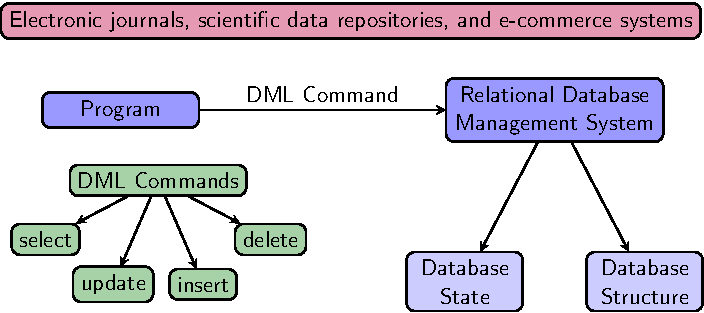
\includegraphics[width=.95\linewidth]{evolution_database_applications_wrapper_crop}
            \vspace*{.05in}
	    \caption{Common Architecture of Many Real-World
              Applications That Interact with a Relational Database.}
            
	  \end{figure}
          \vspace*{-.2in}

      	  \begin{itemize}
          
            \item Silberschatz et al.\ observe that ``practically all
              use of databases occurs from within application
              programs'' \mbox{[Data. Sys. Conc. 2010]}

            \item Database applications rapidly evolve as changes are
              made to both the program and the database's state and
              structure

%% Moreover, many database applications rapidly evolve as software
%% developers change the source code, database administrators modify the
%% database's schema, and external application programs add data to and
%% delete data from the database.
          
          \end{itemize}

        \end{block}

	%%%%%%%%%%%%%%%%%%%%%%%%%%%%%%%%%%%
	%
	% Types of Database Applications
	%
	%%%%%%%%%%%%%%%%%%%%%%%%%%%%%%%%%%%
	\begin{block}{\textsc{Types of Database Applications}}

          \begin{figure}			
  	    \centering
            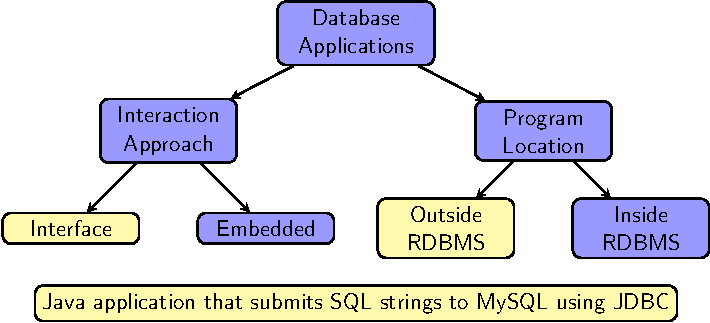
\includegraphics[width=.95\linewidth]{categorize_database_applications_wrapper_crop}
            \vspace*{.05in}
	    \caption{Categorizing Database Applications --- the Presented Method Focuses on the Highlight Type of Application.}

	  \end{figure}
          \vspace*{-.2in}

   	\end{block}

	%%%%%%%%%%%%%%%%%%%%%%%%%%%%%%%%%%%
	%
	% Test Suite Reduction's Role
	%
	%%%%%%%%%%%%%%%%%%%%%%%%%%%%%%%%%%%
   	\begin{block}{\textsc{The Role of Test Suite Reduction}}

          \begin{figure}			
  	    \centering
            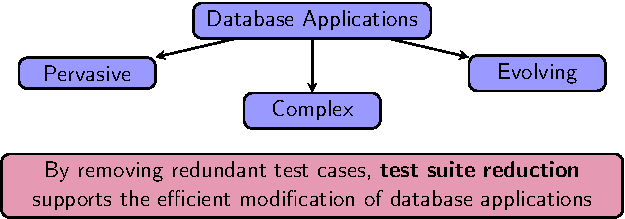
\includegraphics[width=.95\linewidth]{test_suite_reduction_rescue_wrapper_crop}
            \vspace*{.05in}
	    \caption{Test Suite Reduction Aims to Improve the
              Efficiency of Testing Database Applications.}
            
	  \end{figure}          

	\end{block}
      \end{column}   
      
%%%%%%%%%%%%%%%%%%%%%%%%%%%%%%%%%%%%%%%%%%%%%%%%%%%%%%%%%%%%%%%%%%%%%      
%
% Center column
%
%%%%%%%%%%%%%%%%%%%%%%%%%%%%%%%%%%%%%%%%%%%%%%%%%%%%%%%%%%%%%%%%%%%%%
      \begin{column}{.325\linewidth}
   		
	%%%%%%%%%%%%%%%%%%%%%%%%%%%%%%%%%%%
	%
	% Datatabase-Aware Coverage
	%
	%%%%%%%%%%%%%%%%%%%%%%%%%%%%%%%%%%%
	\begin{block}{\textsc{Database-Aware Test Suite Reduction}}

          \begin{figure}			
  	    \centering
            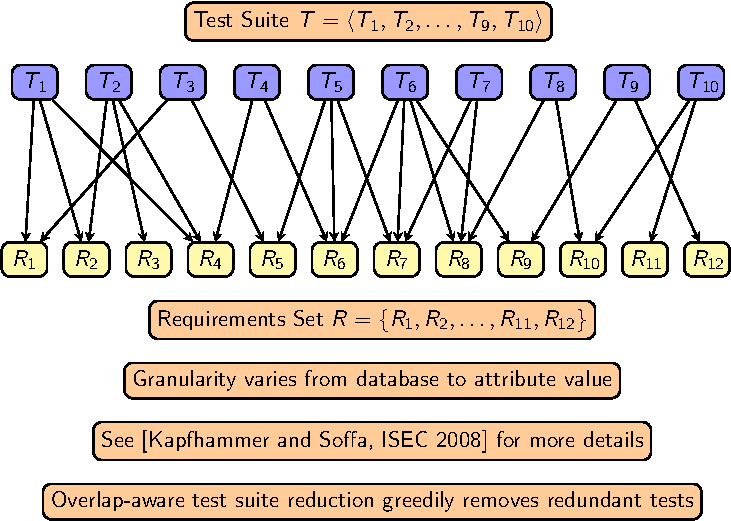
\includegraphics[width=.95\linewidth]{test_coverage_monitoring_wrapper_crop}
            \vspace*{.05in}
	    \caption{The Process of Test Suite Reduction for Database Applications.}
            
	  \end{figure}          

	\end{block}
		
	%%%%%%%%%%%%%%%%%%%%%%%%%%%%%%%%%%%
	%
	% The Case Study Applications
	%
	%%%%%%%%%%%%%%%%%%%%%%%%%%%%%%%%%%%		
	\begin{block}{\textsc{Case Study Applications}}
          
            %% \begin{tabular}{c}

%% \begin{minipage}{.5\linewidth}

\vspace*{-.1in}

\begin{center}
\begin{table}[h]

\begin{center}

\begin{tabular}{r | c | c | c | l} 

{\bf Name} & {\bf Classes} & {\bf Methods} & {\bf NCSS} & {\bf Per} \\
\hline

{Reminder} ({RM}) 
& 9               & 55.0          & 548.0       & {\em Program}
\\ \hline

         &                 & 6.11          & 60.89       & {\em Class}
\\ \hline

         &                 &               & 9.96       & {\em Method} 
\\ [.01in] \hline \hline 

\rule{-.1in}{20pt}

{FindFile} ({FF})
 & 5               & 49.0          & 558.0       & {\em Program}
\\ \hline

         &                 & 9.8           & 111.6       & {\em Class}
\\ \hline

         &                 &               & 11.39       & {\em Method} 
\\ [.01in] \hline \hline 

\rule{-.1in}{20pt}

{Pithy} ({PI}) 
& 11              & 73.0          & 579.0       & {\em Program}
\\ \hline

         &                 & 6.64          & 52.64       & {\em Class}
\\ \hline

         &                 &               & 7.93       & {\em Method} 
\\ [.01in] \hline \hline 
\rule{-.1in}{20pt}

%% \end{tabular}

%% \end{center}

%% \vspace*{-.1in}

%% %% \caption{High Level Description of the {\tt RM}, {\tt FF}, and {\tt
%% %% PI} Case Study Applications.}

%% \label{fig:characterize_first}

%% \end{table} 

%% %% \end{minipage} \\ 

%% %% \begin{minipage}{.5\linewidth}

%% \begin{table}[h]

%% \begin{center}

%% \begin{tabular}{r | c | c | c | l} 

%% {\bf Name} & {\bf Classes} & {\bf Methods} & {\bf NCSS} & {\bf Per} 
%% \\ \hline

{StudentTracker} ({ST})
& 9               & 72.0          & 620.0       & {\em Program}
\\ \hline

         &                 & 8.0           & 68.89       & {\em Class}
\\ \hline

         &                 &               & 8.61        & {\em Method} 
\\ [.01in] \hline \hline 

\rule{-.1in}{20pt}

{TransactionManager} ({TM})
& 6               & 87.0          & 748.0       & {\em Program}
\\ \hline

         &                 & 14.5          & 124.67      & {\em Class}
\\ \hline

         &                 &               & 8.6         & {\em Method} 
\\ [.01in] \hline \hline 

\rule{-.1in}{20pt}

{GradeBook} ({GB})
& 10              & 147.0         & 1455.0       & {\em Program}
\\ \hline

         &                 & 14.7          & 145.5        & {\em Class}
\\ \hline

         &                 &               & 9.9          & {\em Method} \\
%\\ [.1in] \hline \hline 
%\rule{-.1in}{20pt}

\end{tabular}

\end{center}

\vspace*{.1in}

\caption{High-Level Description of the Case Study Applications Used in the Empirical Study.}

\vspace*{-.35in}

\label{fig:characterize_second}

\end{table}
\end{center}

%% \end{minipage}

%% \end{tabular}

            
	  \end{block}
	\end{column}

%%%%%%%%%%%%%%%%%%%%%%%%%%%%%%%%%%%%%%%%%%%%%%%%%%%%%%%%%%%%%%%%%%%%%      
%
% Right column
%
%%%%%%%%%%%%%%%%%%%%%%%%%%%%%%%%%%%%%%%%%%%%%%%%%%%%%%%%%%%%%%%%%%%%%      		
      \begin{column}{.325\linewidth}	
		
	%%%%%%%%%%%%%%%%%%%%%%%%%%%%%%%%%%%
	%
	% The Empirical Results
	%
	%%%%%%%%%%%%%%%%%%%%%%%%%%%%%%%%%%%
        \begin{block}{\textsc{Experimental Results}}

          \vspace*{-.25in}

\begin{table}[h]

\begin{center}

\begin{tabular}{r || c | c | c | c || c} 

  {\bf A - $|T|$} & {\bf Rel.} & {\bf Attrib.} & {\bf Rec.} & 
    {\bf Attrib. Val.} & {\bf All} \\ \hline \hline

  RM - 13  &  (7, .46)   &  (7, .46)  
                 &  (10, .3)     &  (9, .31) & 
                 (8.25, .37) \\ \hline

  FF - 16  &  (7, .56)      &  (7, .56)  
                 &  (11, .31)     &  (11, .31) & 
                 (9, .44) \\ \hline

  PI - 15  &  (6, .6)         &  (6, .6)  
                 &  (8, .7)         &  (7, .53) & 
                 (6.75, .55) \\ \hline

  ST - 25 &  (5, .80)         &  (5, .76)  
                 &  (11, .56)       &  (10, .6) & 
                 (7.75, .69) \\ \hline

  TM - 27 &  (14, .48)      &  (14, .48)  
                 &  (15, .45)      &  (14, .48) & 
                 (14.25, .47) \\ \hline

  GB - 51  &  (33, .35)      &  (33, .35)  
                 &  (33, .35)      &  (32, .37) & 
                 (32.75, .36) 
                 \\ \hline \hline

                 {All} - 24.5  &  (12, .51)           &  (12.17, .5)  
                    &  (14.67, .4)      &  (13.83, .44) & 
                    %$(13.167, .4625)$ 
                %\\ \hline
 
\end{tabular} 

\end{center}

\caption{The Reduction in Test Suite Size for the Database
  Applications with $(|T'|, \mbox{RFFS}(T, T'))$ for All Data Points.}
\label{fig:reductions}
\vspace*{-.1in}

\end{table}


          \vspace*{-.5in}          

          \begin{itemize}

            \item $\mbox{RFFS}(T, T') = (|T|-|T'|) \div |T|$

            \item ST has the best RFFS (.69 avg) and GB has the worst
              (.36 avg)

            \item Across all of the applications, RFFS was .51 on
              average at the relation level and .44 on average at the
              attribute value level

            \item RFFS drops from .50 to .40 when the reducer analyzes
              at the record level instead of the attribute level

            \item RFFS climbs to .44 from .40 with attribute value
              requirements

          \end{itemize}

          \vspace*{.1in}

          \vspace*{-.25in}

\begin{table}[h]

\begin{center}

\begin{tabular}{r || c | c | c | c || c} 

  {\bf Application } & {\bf Relation} & {\bf Attribute} & {\bf Record} & 
  {\bf Attribute Value} & {\bf All} \\ \hline \hline

  RM  & .07  & .07 & .04 & .05 & .07

  \\ \hline

  FF  & .13 & .13 & .08 & .08 & .11

  \\ \hline

  PI & .29 & .29 & .15 & .18 & .23

  \\ \hline

  ST & .19 & .18 & .13 & .13 & .16

  \\ \hline

  TM & .23 & .23 & .19 & .22 & .22

  \\ \hline

  GB & .78 & .78 & .78 & .78 & .78 
        
  \\ \hline \hline

  {All} & .28 & .28 & .23 & .24  & 
 
\end{tabular} 

\end{center}

\caption{The Reduction in Test Suite Time for the Database
  Applications with $\mbox{RFFT}(T, T')$ for All Data Points.}
\label{fig:reductions}
\vspace*{-.1in}

\end{table}
          

          \vspace*{-.5in}          

          \begin{itemize}

            \item $\mbox{RFFT}(T, T') = (\mbox{{\em time}}(T)-\mbox{{\em
                time}}(T')) \div \mbox{{\em time}}(T)$

            \item GB has the highest RFFT value because it contains
              redundant tests that restart the database and are thus
              very costly to run

            \item Except for GB, the RFFT values are lower than those
              for RFFS

            %% \item For all of the applications, RFFS was .28 on average
            %%   at the relation level and .24 on average at the
            %%   attribute value level

            \item RFFS was .28 on average at the relation level and
              .24 on average at the attribute value level, across all
              of the applications

            %% \item RFFS decreases from .28 to .23 when the reducer
            %%   analyzes at the record level instead of the attribute
            %%   level

            \item When the reducer analyzes at the record level
              instead of the attribute value level, RFFS decreases
              from .28 to .23

            \item With attribute value requirements RFFS increases to
              .24 from .23

          \end{itemize}

	\end{block}	    

	%%%%%%%%%%%%%%%%%%%%%%%%%%%%%%%%%%%
	%
	% Future Work
	%
	%%%%%%%%%%%%%%%%%%%%%%%%%%%%%%%%%%%				
	\begin{alertblock}{\textsc{Future Work}}
          \begin{itemize}
	  \item Use larger and more varied applications in follow-on experiments
	  \item Investigate the fault-detection effectiveness of $T$ and $T'$
	  \item Focus on affiliated testing tasks (e.g., test data generation)
	  \end{itemize}
	\end{alertblock}
      \end{column}
      
	\end{columns}
  \end{frame}
\end{document}
